\documentclass[tikz,border=5pt]{standalone}
\usepackage{amsmath}
\usepackage{xcolor}
\usetikzlibrary{arrows.meta,backgrounds,calc,fit,positioning}
\definecolor{ink}{HTML}{0F172A}
\definecolor{mutedInk}{HTML}{475569}
\definecolor{lineGray}{HTML}{CBD5E1}
\definecolor{panelGray}{HTML}{F8FAFC}
\definecolor{summaryGray}{HTML}{F1F5F9}
\definecolor{operationTeal}{HTML}{0F766E}
\definecolor{operationFill}{HTML}{ECFEFF}
\definecolor{schemaViolet}{HTML}{6D28D9}
\definecolor{schemaFill}{HTML}{F5F3FF}
\definecolor{resultGreen}{HTML}{15803D}
\definecolor{resultFill}{HTML}{F0FDF4}

\tikzset{
  state card/.style={
    draw=mutedInk,
    fill=white,
    rounded corners=1.5mm,
    line width=0.55pt,
    font=\sffamily\small,
    align=center,
    inner sep=3mm,
    text=ink
  },
  concept card/.style={
    state card,
    fill=panelGray
  },
  summary card/.style={
    state card,
    fill=summaryGray
  },
  operation card/.style={
    draw=operationTeal,
    fill=operationFill,
    rounded corners=4mm,
    line width=0.75pt,
    font=\sffamily\small\bfseries,
    align=center,
    inner xsep=4mm,
    inner ysep=2.2mm,
    text=operationTeal
  },
  schema ref/.style={
    draw=schemaViolet,
    fill=schemaFill,
    double=schemaViolet,
    double distance=1pt,
    rounded corners=1mm,
    line width=0.65pt,
    font=\sffamily\bfseries,
    inner xsep=5mm,
    inner ysep=2.5mm,
    text=schemaViolet
  },
  result card/.style={
    state card,
    draw=resultGreen,
    fill=resultFill,
    text=resultGreen,
    line width=0.75pt
  },
  bank card/.style={
    draw=schemaViolet,
    fill=white,
    rounded corners=2mm,
    line width=0.75pt,
    inner sep=4mm,
    text=ink
  },
  meta edge/.style={
    -{Stealth[length=2mm]},
    densely dashed,
    draw=mutedInk,
    line width=0.6pt
  },
  process edge/.style={
    -{Stealth[length=2.2mm]},
    draw=ink,
    line width=0.85pt
  },
  section label/.style={
    font=\sffamily\scriptsize\bfseries,
    text=mutedInk,
    align=left
  }
}


\begin{document}
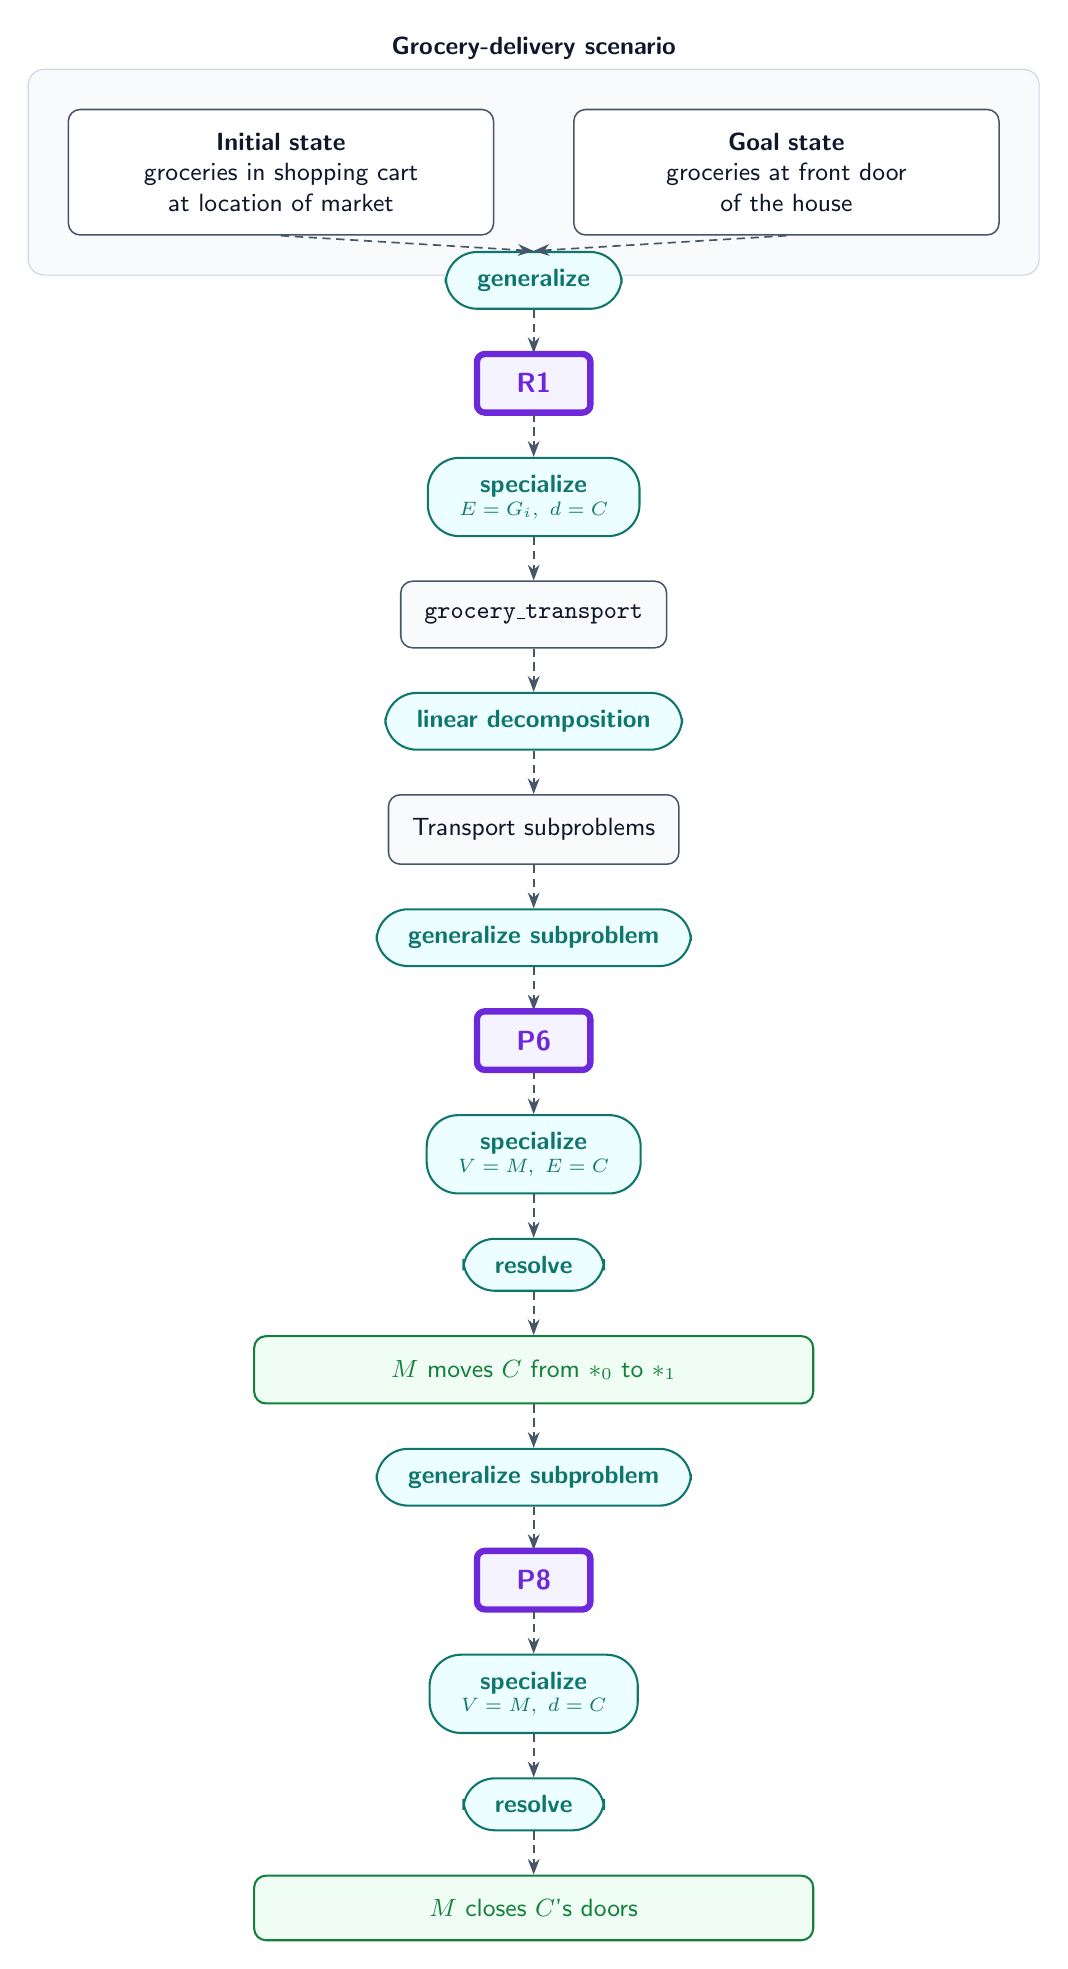
\begin{tikzpicture}[node distance=5.5mm]
  \node[state card,text width=48mm] (initial) {
    \textbf{Initial state}\\
    groceries in shopping cart\\
    at location of market
  };
  \node[state card,text width=48mm,right=10mm of initial] (goal) {
    \textbf{Goal state}\\
    groceries at front door\\
    of the house
  };
  \begin{scope}[on background layer]
    \node[draw=lineGray,fill=panelGray,rounded corners=2mm,
          fit=(initial)(goal),inner sep=5mm,
          label={[font=\sffamily\small\bfseries,text=ink]above:Grocery-delivery scenario}] (scenario) {};
  \end{scope}

  \coordinate (problem-center) at ($(initial)!0.5!(goal)$);
  \node[operation card,below=10mm of problem-center] (generalize-r1) {generalize};
  \node[schema ref,below=of generalize-r1] (r1) {R1};
  \node[operation card,below=of r1] (specialize-r1) {
    specialize\\[-1mm]
    \scriptsize $E=G_i,\ d=C$
  };
  \node[concept card,below=of specialize-r1] (transport) {\texttt{grocery\_transport}};
  \node[operation card,below=of transport] (decompose) {linear decomposition};
  \node[concept card,below=of decompose] (subproblems) {Transport subproblems};

  \node[operation card,below=of subproblems] (generalize-p6) {generalize subproblem};
  \node[schema ref,below=of generalize-p6] (p6) {P6};
  \node[operation card,below=of p6] (specialize-p6) {
    specialize\\[-1mm]
    \scriptsize $V=M,\ E=C$
  };
  \node[operation card,below=of specialize-p6] (resolve-move) {resolve};
  \node[result card,text width=65mm,below=of resolve-move] (move) {
    $M$ moves $C$ from $*_0$ to $*_1$
  };

  \node[operation card,below=of move] (generalize-p8) {generalize subproblem};
  \node[schema ref,below=of generalize-p8] (p8) {P8};
  \node[operation card,below=of p8] (specialize-p8) {
    specialize\\[-1mm]
    \scriptsize $V=M,\ d=C$
  };
  \node[operation card,below=of specialize-p8] (resolve-doors) {resolve};
  \node[result card,text width=65mm,below=of resolve-doors] (close) {
    $M$ closes $C$'s doors
  };

  \draw[meta edge] (initial.south) -- (generalize-r1.north);
  \draw[meta edge] (goal.south) -- (generalize-r1.north);
  \draw[meta edge] (generalize-r1) -- (r1);
  \draw[meta edge] (r1) -- (specialize-r1);
  \draw[meta edge] (specialize-r1) -- (transport);
  \draw[meta edge] (transport) -- (decompose);
  \draw[meta edge] (decompose) -- (subproblems);
  \draw[meta edge] (subproblems) -- (generalize-p6);
  \draw[meta edge] (generalize-p6) -- (p6);
  \draw[meta edge] (p6) -- (specialize-p6);
  \draw[meta edge] (specialize-p6) -- (resolve-move);
  \draw[meta edge] (resolve-move) -- (move);
  \draw[meta edge] (move) -- (generalize-p8);
  \draw[meta edge] (generalize-p8) -- (p8);
  \draw[meta edge] (p8) -- (specialize-p8);
  \draw[meta edge] (specialize-p8) -- (resolve-doors);
  \draw[meta edge] (resolve-doors) -- (close);
\end{tikzpicture}
\end{document}
